\chapter{Use Case 1: WorldData}
\label{worlddata}

\section{Einführung}
Im ersten Use Case geht es hauptsächlich um die Anzeige grosser Datenmengen auf der Karte. Dazu importieren wir bestehende Datenbestände in die Google Fusion Tables und visualisieren diese mittels Google Maps API auf der Karte.

\subsection{Ziel}
Es sollen verschiedene historische Länderdaten auf einer Weltkarte angezeigt werden. Die Daten sind pro Jahr und Thema unterteilt. Über eine Zeitachse soll es möglich sein die Daten der verschiedenen Jahre zu selektieren. Eine solche Darstellung kann beispielsweise dabei helfen Zusammenhänge zwischen verschiedenen Themenbereichen zu finden.

\subsection{Vorgehen}
Um die Daten pro Land zu visualisieren, werden zuerst die Landesgrenzen als Geometrie-Datensätze in eine separate Fusion Tabelle importiert. In eine andere Tabelle werden dann die Daten importiert unterteilt nach Land und Jahr. Diese beiden Tabellen werden per Merge-Funktion zu einer Tabelle zusammengefasst, welche dann mittels FusionTablesLayer des Google Maps APIs auf der Karte dargestellt werden kann.

\subsection{Datenquellen}
Als Datenquelle wurde der Daten Katalog der Weltbank\footnote{\url{http://data.worldbank.org/}} verwendet. Darin finden sich länderspezifische Daten aufgeteilt in über 7000 Themenbereiche. Diese lassen sich als XML- oder Excel-Datei herunterladen. Für unseren Import verwendeten wir die Excel-Dateien, welche wir vorbereitet und als CSV-Dateien gespeichert haben. Diese konnten wir als neue Google Fusion Tables importieren.

Die Landesgrenzen wurden als \gls{KML}-Datei von einer inoffiziellen Google Earth Library-Webseite\footnote{\url{http://www.gelib.com/world-borders.htm}} bezogen. 

\section{Analyse}
\todo[inline]{UseCase 1: WorldData - Analyse}

\section{Design}

\subsection{UseCases}

\begin{figure}[h!]
	\centering
	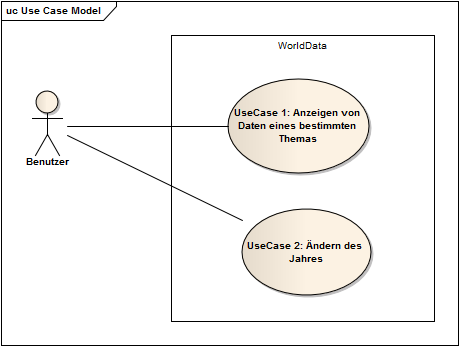
\includegraphics[scale=0.8]{images/usecase1-worlddata/uml/worlddata-usecasemodel.png}
	\caption{WorldData UseCase Modell}
	\label{worlddata-usecasemodel}
\end{figure}

% Use Case 1: Anzeigen von Daten eines bestimmten Themas
\subsubsection{Use Case 1: Anzeigen von Daten eines bestimmten Themas}
\paragraph{Primary Actor}
\begin{itemize}
\item Benutzer
\end{itemize}

\paragraph{Stakeholders and Interests}
\begin{itemize}
\item Benutzer: Möchte Daten zu einem bestimmten Thema auf der Karte anzeigen
\end{itemize}

\paragraph{Preconditions}
\begin{itemize}
\item Webapplikation ist gestartet
\end{itemize}

\paragraph{Success Guarantee (Postconditions)}
\begin{itemize}
\item Daten des gewählten Themas werden auf der Karte angezeigt
\item Legende zu den Daten wird angezeigt
\end{itemize}

\paragraph{Main Success Scenario}
\begin{enumerate}
\item Benutzer wählt das Thema aus
\end{enumerate}

\paragraph{Special Requirements}
-

\paragraph{Frequency of Occurrence}
Tritt sehr häufig auf, da eine beliebige Anzahl von Benutzern die Webapplikation bedienen können.

% Use Case 2: Ändern des Jahres
\subsubsection{Use Case 2: Ändern des Jahres}
\paragraph{Primary Actor}
\begin{itemize}
\item Benutzer
\end{itemize}

\paragraph{Stakeholders and Interests}
\begin{itemize}
\item Benutzer: Möchte Daten eines anderen Jahres anzeigen
\end{itemize}

\paragraph{Preconditions}
\begin{itemize}
\item Webapplikation ist gestartet
\item Thema ist ausgewählt
\end{itemize}

\paragraph{Success Guarantee (Postconditions)}
\begin{itemize}
\item Daten des gewählten Jahres werden auf der Karte angezeigt
\end{itemize}

\paragraph{Main Success Scenario}
\begin{enumerate}
\item Benutzer wählt das gewünschte Jahr aus
\end{enumerate}

\paragraph{Alternative Flows}
1a. Falls für das gewählte Jahr keine Daten vorhanden sind, ist dies ebenfalls auf der Karte ersichtlich.

\paragraph{Special Requirements}
-

\paragraph{Frequency of Occurrence}
Tritt sehr häufig auf, da eine beliebige Anzahl von Benutzern die Webapplikation bedienen können.

\subsection{ERD}
\begin{figure}[!h]
	\centering
	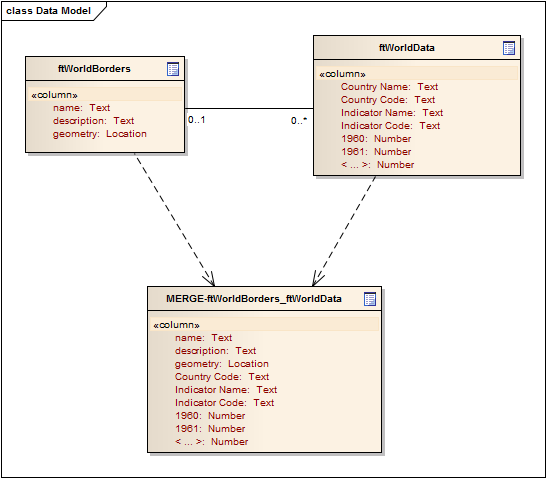
\includegraphics[scale=0.8]{images/usecase1-worlddata/uml/worlddata-erd.png}
	\caption{WorldData ERD}
	\label{worlddata-erd}
\end{figure}

\subsection{Klassendiagramm}
\begin{figure}[!h]
	\centering
	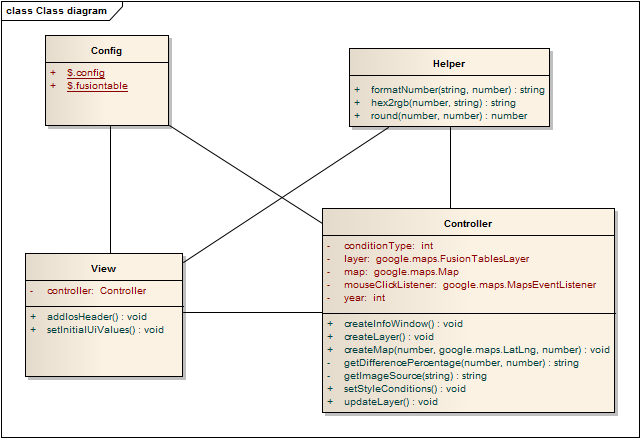
\includegraphics[scale=0.7]{images/usecase1-worlddata/uml/worlddata-classdiagram.png}
	\caption{WorldData Klassendiagramm}
	\label{worlddata-classdiagram}
\end{figure}

\section{Implementation}
Die Applikation wurde als Webapplikation implementiert. Für die GUI-Elemente wurde das Javascript Framework jQuery Mobile verwendet. Dieses bietet eine sehr grosse Plattform-Unterstützung, was im Webbereich sehr wichtig ist.

\subsection{Systemanforderungen:}
Da es sich um eine Webapplikation handelt, ist es möglich die Applikation auf beinahe allen Geräten, welche über einem Browser verfügen zu starten. Einschränkungen gibt es nur in den unterstützten Browsern. Eine Liste davon findet sich auf der Webseite des jQuery Mobile Frameworks:  \url{http://jquerymobile.com/blog/2012/04/06/jquery-mobile-1-1-0-rc2/#platforms}

\subsection{Abhängigkeiten}
\begin{tabular}{|l|l|p{8cm}|}
\hline 
\textbf{Library} & \textbf{Version} & \textbf{Verwendung} \\ 
\hline 
jQuery Mobile & 1.1.0 & GUI-Elemente \\ 
\hline 
jQuery & 1.7.1 & Basis für den Gebrauch von jQuery Mobile \\ 
\hline 
Google Maps API & V3 & Karte mit FusionTablesLayer \\ 
\hline 
Cubiq - Add to home screen & 2.0 & Popup welches auf allen iOS Geräten erscheint \\ 
\hline 
\end{tabular} 

\subsection{Quellcode-Struktur}
\begin{tabular}{|l|l|}
\hline 
\textbf{Datei} & \textbf{Beschreibung} \\ 
\hline 
images/ & Bilder der Applikation \\ 
\hline 
js/ & JavaScripts der Applikation \\ 
\hline 
js/Config.js & Konfiguration der Applikation \\ 
\hline 
js/Controller.js & Controller der Applikation \\ 
\hline 
js/Helper.js & Helper-Funktionen welche von der Applikation verwendet werden \\ 
\hline 
js/View.js & Steuert die Anzeige der Applikation \\ 
\hline 
lib/ & Von der Applikation verwendete Libraries \\ 
\hline 
styles/ & CSS-Styles der Applikation \\ 
\hline
index.html & Startseite der Applikation \\ 
\hline
\end{tabular} 

\section{Test}
\todo[inline]{UseCase 1: WorldData - Test}

\section{Resultate}
Das FusionTablesLayer Element der Google Maps API eignet sich sehr gut zur Darstellung einer grossen Anzahl von Daten. Leider hindern die Einschränkungen betreffend Styles (siehe \ref{fusiontableslayer-styles-restrictions}) stark den individuellen Gestalltungsprozess der Ebene.

Wie wir feststellen mussten, sind diese 5 Stile sehr schnell aufgebraucht. Einer davon fällt meistens für den Standard-Stil weg. Dieser wird angewendet, wenn die entsprechende Zeile aus der Tabelle auf keine Bedingung der restlichen Stile passt. So bleiben lediglich noch 4 Stile übrig für alle Elemente die man speziell hervorheben möchte.

Sobald man dann auch noch verschiedene Geometrie-Typen in der Tabelle abgelegt hat (Punkt, Linie, Fläche), muss man sich gut überlegen, für welche Elemente man wirklich einen speziellen Stil anwenden will.

\section{Weiterentwicklung}
Da es sich bei der Applikation lediglich um einen Prototypen handelt, bietet diese natürlich noch ein grosses Potential zur Weiterentwicklung. Hier eine Auflistung möglicher Features, welche noch implementiert werden könnten:

\begin{itemize}
\item Weitere Themen in die Datenbank importieren
\item Auswahl der Länder für welche Daten angezeigt werden sollen
\item Anzeige einer Rangliste der 10 Länder mit den höchsten Werten des gewählten Themas
\item Direkter Vergleich verschiedener Länder
\end{itemize}


\section{Benutzerdokumentation}
\subsection{Importieren der Daten in Google Fusion Tables}

\subsubsection{Landesgrenzen}
\label{landesgrenzen}
Die Landesgrenzen liegen als KML-Datei vor. Diese beinhaltet alle Länder mit ihren Grenzen definiert als Polygone.

\begin{figure}[!h]
	\centering
	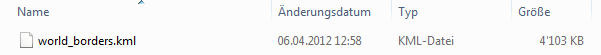
\includegraphics{images/usecase1-worlddata/documentation/worlddata-worldborders_kml.png}
	\caption{WorldData Landesgrenzen liegen als KML-Datei vor}
	\label{worlddata-worldborders_kml}
\end{figure}

\begin{enumerate}
\item Google Docs öffnen (\url{https://docs.google.com/}) und sich mit seinem Google Account einloggen
\item Erstellen > Tabelle (Beta) \\ 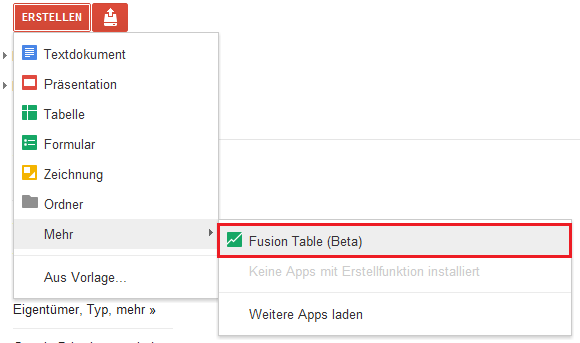
\includegraphics{images/usecase1-worlddata/documentation/worlddata-worldborders_import1.png}
\item Es öffnet sich die neue Fusion Table mit dem Dialog zum Importieren von bestehenden Daten
\item Im Tab \emph{From this computer} die lokal gespeicherte Datei auswählen > Next
\item Die Daten werden automatisch in passende Spalten eingeteilt
\item Abschliessend muss der Tabelle noch einen Namen gegeben werden
\item Mit \emph{Finish} werden die Daten dann importiert
\end{enumerate}

Die Tabelle sollte nun folgendermassen aussehen:

\begin{figure}[!h]
	\centering
	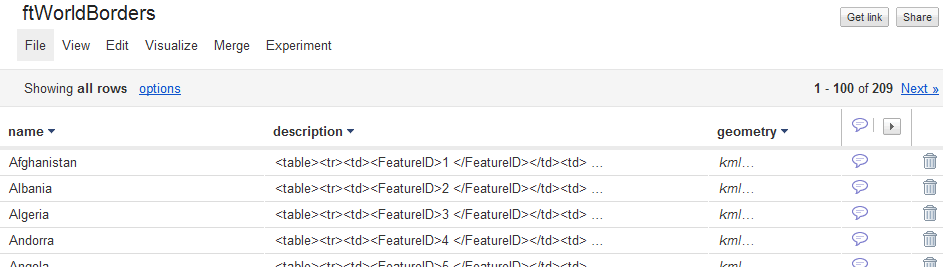
\includegraphics[scale=0.65]{images/usecase1-worlddata/documentation/worlddata-worldborders_import_done.png}
	\caption{WorldData Landesgrenzen erfolgreich als Fusion Table importiert}
	\label{worlddata-worldborders_import_done}
\end{figure}

\subsubsection{Daten}
Die Daten liegen als CSV-Datei vor. Diese beinhaltet folgende Spalten:
\begin{itemize}
\item Country Name
\item Country Code
\item Indicator Name
\item Indicator Code
\item 1960
\item 1961
\item ...
\end{itemize}

\begin{figure}[!h]
	\centering
	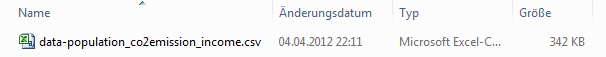
\includegraphics{images/usecase1-worlddata/documentation/worlddata-data_csv.png}
	\caption{WorldData Daten liegen als CSV-Datei vor}
	\label{worlddata-data_csv}
\end{figure}

Das Vorgehen für den Import der Daten ist dasselbe wie bei den Landesgrenzen (\ref{landesgrenzen}).

Nach dem Import der Daten sollte die Tabelle folgendermassen aussehen:

\begin{figure}[!h]
	\centering
	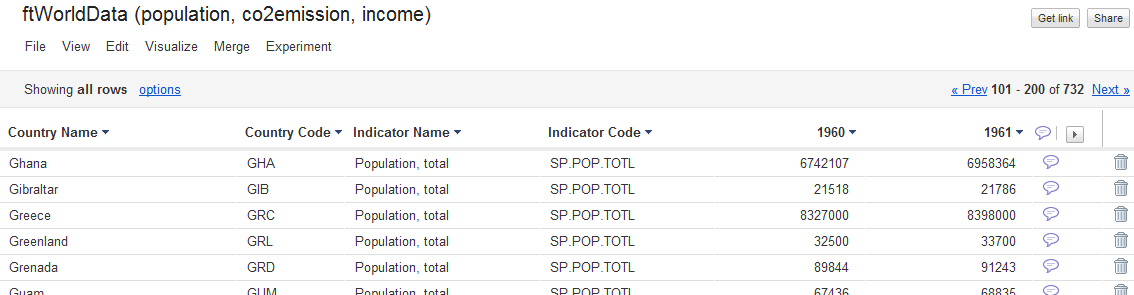
\includegraphics[scale=0.5]{images/usecase1-worlddata/documentation/worlddata-data_import_done.png}
	\caption{WorldData Daten erfolgreich als Fusion Table importiert}
	\label{worlddata-data_import_done}
\end{figure}

\subsubsection{Tabellen mergen}
Sind beide Fusion Tables erstellt müssen diese zusammengefügt werden, um sie schlussendlich als einen einzelnen Layer auf der Karte darzustellen. Dazu bietet Google Fusion Tables die \emph{Merge}-Funktion an. 

\begin{enumerate}
\item Eine der beiden Tabellen öffnen
\item Im Menü \emph{Merge} auswählen \\ 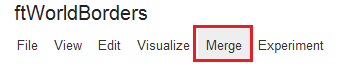
\includegraphics{images/usecase1-worlddata/documentation/worlddata-merge1.png}
\item Es öffnet sich ein Popup, welches durch den Vorgang führt
\item In der 1. Spalte wählt man die Spalte aus, über welche die beiden Tabellen verbunden werden sollen. In unserem Fall ist dies die Spalte mit den Namen der Länder.
\item In der 2. Spalte muss man zuerst die andere Tabelle auswählen und dann ebenfalls die Spalte, in welcher die Namen der Länder gespeichert sind.
\item Schlussendlich muss der neuen Tabelle ein Namen gegeben werden
\item Mit einem Klick auf \emph{Merge tables} wird die neue Tabelle mit den zusammengefügten Daten erstellt. \\ 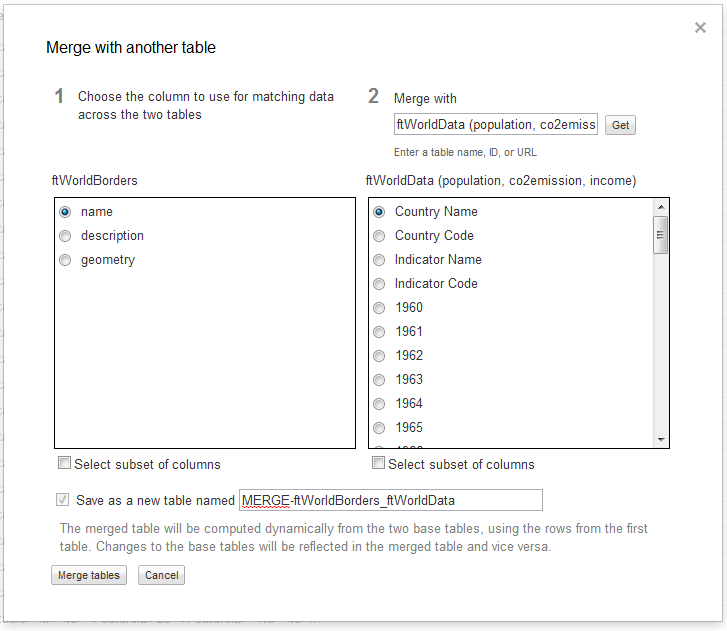
\includegraphics[scale=0.8]{images/usecase1-worlddata/documentation/worlddata-merge2.png}
\end{enumerate}

Die zusammengeführte Tabelle sollte nun folgendermassen aussehen:

\begin{figure}[!h]
	\centering
	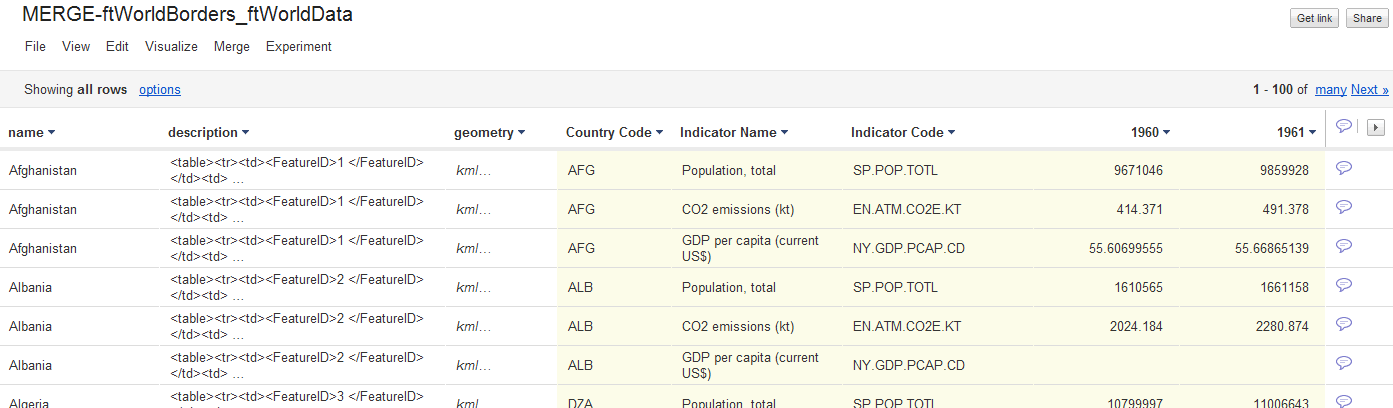
\includegraphics[scale=0.4]{images/usecase1-worlddata/documentation/worlddata-merge_done.png}
	\caption{WorldData Merge der Landesgrenzen- und Daten-Tabelle}
	\label{worlddata-merge_done}
\end{figure}

\subsubsection{Merge-Tabelle für die Verwendung mit FusionTablesLayer vorbereiten}
Um die Tabelle nun als FusionTablesLayer verwenden zu können, muss diese als \emph{öffentlich} markiert werden. Dazu klickt man bei der geöffneten Tabelle auf den \emph{Share}-Button in der linken oberen Ecke.

\begin{figure}[!h]
	\centering
	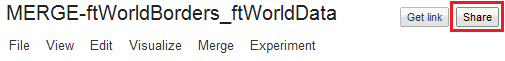
\includegraphics{images/usecase1-worlddata/documentation/worlddata-prepare_fusiontableslayer1.png}
	\caption{WorldData Freigabe der Merge-Tabelle}
	\label{worlddata-prepare_fusiontableslayer1}
\end{figure}

Im Dialogfenster wählt man unter \emph{Visibility options} den Eintrag \emph{Public} aus.

\begin{figure}[!h]
	\centering
	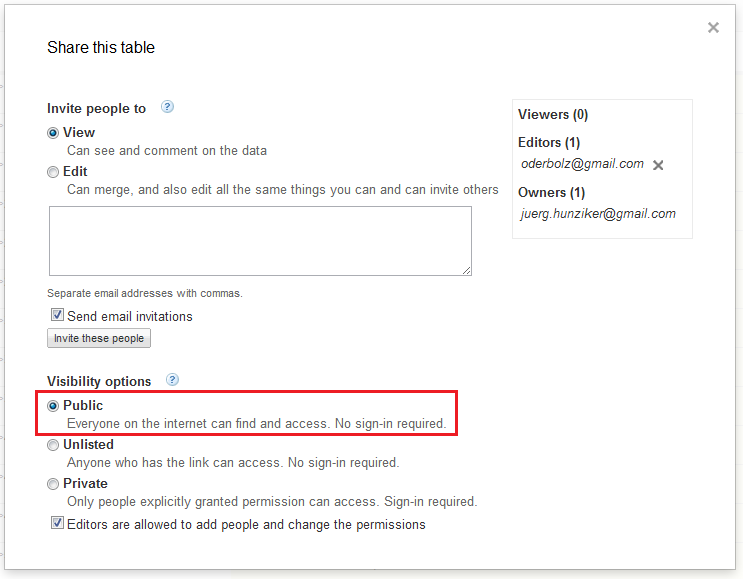
\includegraphics[scale=0.5]{images/usecase1-worlddata/documentation/worlddata-prepare_fusiontableslayer2.png}
	\caption{WorldData Freigabeeinstellungen der Merge-Tabelle}
	\label{worlddata-prepare_fusiontableslayer2}
\end{figure}

Als letzten Schritt muss man sich noch die eindeutige ID der Tabelle merken. Dazu wählt man im Menü  \emph{File > About} und kopiert sich die angezeigte \emph{Encrypted ID} im geöffneten Dialog.

\begin{figure}[!h]
	\centering
	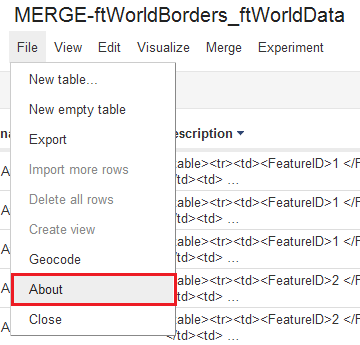
\includegraphics{images/usecase1-worlddata/documentation/worlddata-prepare_fusiontableslayer3.png}
	\caption{WorldData ID der Merge-Tabelle finden}
	\label{worlddata-prepare_fusiontableslayer3}
\end{figure}

\begin{figure}[!h]
	\centering
	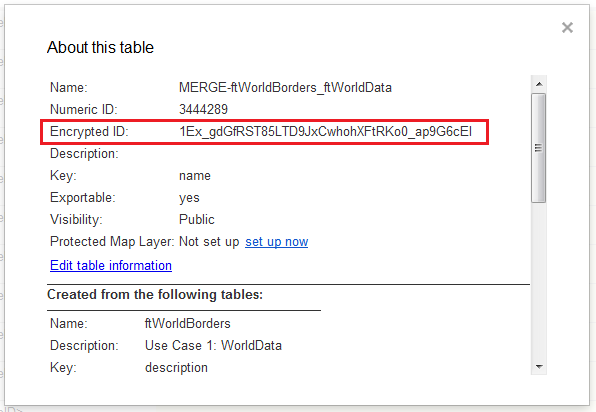
\includegraphics{images/usecase1-worlddata/documentation/worlddata-prepare_fusiontableslayer4.png}
	\caption{WorldData ID der Merge-Tabelle Dialog}
	\label{worlddata-prepare_fusiontableslayer4}
\end{figure}

\subsection{Konfiguration der Applikation}
Um die eben erstellte Fusion Table nun in der WorldData-Applikation zu verwenden muss diese folgendermassen konfiguriert werden.

\subsubsection{/js/Config.js}
\begin{tabular}{|l|l|p{8cm}|}
\hline 
Parameter & Datentyp & Beschreibung \\ 
\hline 
\$.fusiontable.id & int & Öffnetliche ID der zu verwendenden Fusion Table \\ 
\hline 
\$.fusiontable.field & string & Spaltenname welcher die Landesgrenzen speichert

\textit{(ACHTUNG: Gross-/Kleinschreibung relevant)} \\ 
\hline 
\$.fusiontable.typeField & string & Spaltenname aus welchem die Themen gelesen werden sollen

\textit{(ACHTUNG: Gross-/Kleinschreibung relevant)} \\ 
\hline 
\$.fusiontable.types & - & Konfiguration der verschiedenen Themen. Für jedes Thema muss ein neuer Block nach folgendem Schema erstellt werden:

\lstset{language=JavaScript}
\begin{lstlisting}
'<TYPE>': {
	name: '<TYPE.name>',
	styleBoundaries: {
		low: <TYPE.styleBoundaries.low>,
		medium: <TYPE.styleBoundaries.medium>,
		high: <TYPE.styleBoundaries.high>
	}
}
\end{lstlisting} \\ 
\hline 
- TYPE & string & ID des Themas \\ 
\hline 
- TYPE.name & string & Bezeichnung des Themas \\ 
\hline 
- TYPE.styleBoundaries.low & int & Obere Grenze für tiefe Werte \\ 
\hline 
- TYPE.styleBoundaries.medium & int & Obere Grenze für mittlere Werte \\ 
\hline 
- TYPE.styleBoundaries.high & int & Obere Grenze für hohe Werte \\ 
\hline 
\end{tabular}

\subsection{Starten der Applikation}
Beim Starten der Applikation sollten nun alle Themen der angegebenen Fusion Table in das Auswahlfeld \emph{Ebene auswählen...} geladen werden.

\begin{figure}[!h]
	\centering
	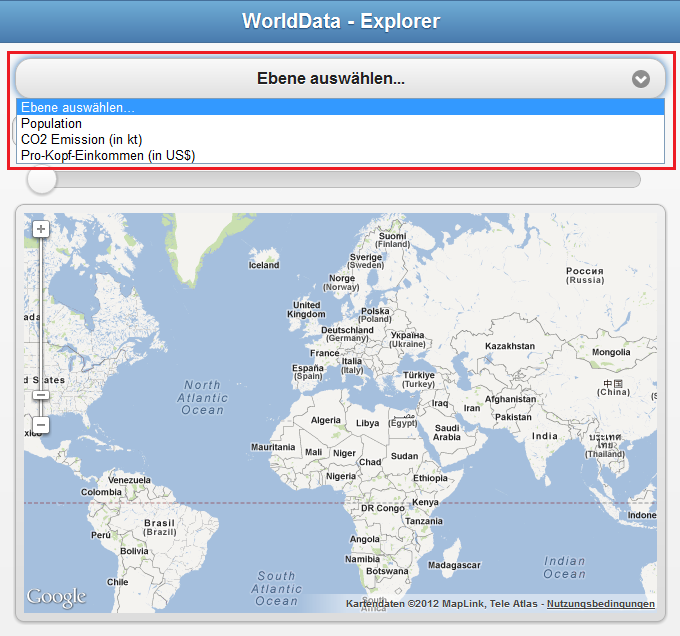
\includegraphics[scale=0.7]{images/usecase1-worlddata/documentation/worlddata-application_start.png}
	\caption{WorldData Auswahlliste der Themen}
	\label{worlddata-application_start}
\end{figure}